\chapter{Social Engineering}
\label{chapter:se}

\section{Definition}

Nach einer groben Definition des Wortes \qqq{Social Engineering} (engl. \qqq{soziale Manipulation})
handelt es sich um eine zwischenmenschliche Beeinflussung durch diverse psychologische
Tricks zweckgemäß konkrete Verhaltensmuster hervorzurufen.
Social Engineering ist also ein Werkzeug, das nicht inhärent gut oder schlecht ist, sondern vielmehr durch seine Anwendung spezifiziert wird.


Geläufiger ist eine Definition im Sinne der Manipulation von Menschen, unrechtmäßig Informationen preiszugeben oder Aktionen auszuführen.
Unter derartige Aktionen fallen beispielsweise das Aushebeln von Sicherheitsfunktionen, das Tätigen von Überweisungen oder
das Installieren von Schadsoftware \bcite{1_enisa,2_bsi}.

Das Bundeskriminalamt legt in einer Forschungsstudie die offizielle Definition des Verfassungsschutzes Brandenburg
zugrunde: \qq{Social Engineering ist der Versuch, unter Ausnutzung menschlicher Eigenschaften Zugang zu Know-how zu erhalten.
Der Angreifer nutzt dabei Dankbarkeit, Hilfsbereitschaft, Stolz, Karrierestreben, Geltungssucht, Bequemlichkeit oder Konfliktvermeidung aus.
Dabei bieten häufig soziale Netzwerke oder auch Firmenwebseiten Möglichkeiten, um sich auf sein Opfer gründlich vorzubereiten.
Zu diesen 'Vorfeldermittlungen' können auch Anrufe im Unternehmen gehören.
Professionelle Angreifer versuchen dabei nicht, mit einem Anruf alle gewünschten Informationen zu erlangen,
dies könnte misstrauisch stimmen. Der Angerufene wird dabei im Gespräch nach vermeintlich nebensächlich erscheinenden Informationen gefragt.}

In der Kurzfassung: Social Engineering ist eine zwischenmenschliche Manipulation,
bei der ein Unbefugter unter Vortäuschung falscher Tatsachen versucht, unberechtigten Zugang zu Informationen oder IT-Systemen zu erlangen \bcite{10_bka}.

In Bezug zu IT-Systemen und digitalen Daten wird Social Engineering auch konkreter als \qqq{Social Hacking} definiert \bcite{deficramer,defidgionos}.

\section{Angriffsvektoren}

\subsection{Methodik}

Obgleich unterschiedliche Social Engineering Angriffe fundamental verschieden ablaufen,
so haben sie dennoch eine grundlegende Struktur gemeinsam.
Diese Struktur lässt sich in vier Phasen einteilen:

\begin{minipage}{.5\linewidth}
    \begin{itemize}
        \setlength\itemsep{1em}
        \item 1) Research
        \item 2) Hook
        \item 3) Play
        \item 4) Out
    \end{itemize}
\end{minipage}
\hfill
\begin{minipage}{.5\linewidth}
    \centering
    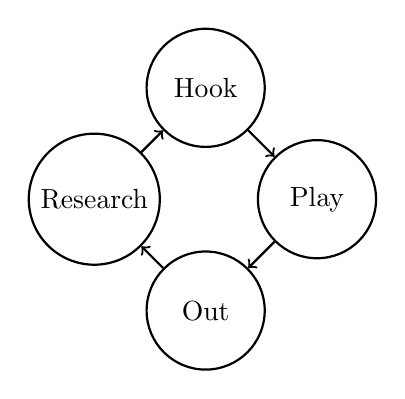
\begin{tikzpicture}[node distance={2cm}, thick, main/.style = {draw, circle, minimum size=15mm}]
        \node[main] (1) {Research};
        \node[main] (2) [above right of=1] {Hook};
        \node[main] (3) [below right of=2] {Play};
        \node[main] (4) [below right of=1] {Out};
        \draw[->] (1) -- (2);
        \draw[->] (2) -- (3);
        \draw[->] (3) -- (4);
        \draw[->] (4) -- (1);
    \end{tikzpicture}
\end{minipage}
\bcite{4_mdpi,cycle,ransomware}

\subsubsection{Research}
In der ersten Phase sucht der Angreifer sein Opfer aus und sammelt alle erwerblichen Informationen
im Zusammenhang mit dieser Person. Anhand dessen kann ein möglicher Angriffsvektor etabliert werden.
Der Erfolg eines Angriffes ist oft abhängig von ausführlicher Recherche, weshalb ein Großteil des zeitlichen
Aufwandes in dieser Phase steckt \bcite{4_mdpi,cycle,ransomware}.

\subsubsection{Hook}
In der \qqq{Hook} Phase baut der Angreifer eine Beziehung mit dem Opfer auf. Die Qualität dieser Beziehung bestimmt
die folgende Kooperation des Opfers. Abhängig von dem exakten Angriffsvektor kann diese Phase beispielsweise
eine langwierige Beziehung durch etwa Social Media darstellen. In anderen Angriffen definiert diese Phase den ersten
Eindruck im Affekt einer Situation, etwa durch freundliche Gestik oder Mimik. Es reichen für die meisten Menschen
bereits 100 ms\footnote{Millisekunden} aus, um über Attraktivität, Sympathie, Vertrauenswürdigkeit, Kompetenz und
Aggressivität zu urteilen \bcite{firstimpression}, weshalb der erste Eindruck bei gewissen Social Engineering
Taktiken elementar ist \bcite{4_mdpi,cycle,ransomware}.

\subsubsection{Play}
In der dritten Phase nutzt der Angreifer die zuvor erlangten Informationen und die Beziehung zum Opfer aus,
um dieses dazu zu bewegen, sensible Daten preiszugeben oder eine sicherheitskritische Aktion auszuführen \bcite{4_mdpi,cycle,ransomware}.

\subsubsection{Out}
Zuletzt zieht sich der Angreifer in der letzten Phase zurück, ohne jegliche Beweise eines Angriffes zurückzulassen.
Zum Beispiel werden digitale Fußabdrücke gelöscht, sodass der Angriff gegebenenfalls nicht auffällt,
die Identität des Angreifers anonym bleibt und die Möglichkeit besteht, zukünftig erneut Kontakt aufzunehmen \bcite{4_mdpi,cycle,ransomware}.

\subsection{Klassifikation}

Social Engineering Angriffe können hinsichtlich verschiedener Aspekte klassifiziert werden\footnote{Social Engineering Angriffe können gegebenenfalls mehrere dieser Aspekte kombinieren.}.
Einerseits lassen sich verschiedene Angriffsvektoren nach dem verwendeten Medium unterscheiden.
Auf diese Weise lassen sich die folgenden zwei Kategorien identifizieren:

\begin{minipage}{.5\linewidth}
    \begin{itemize}
        \setlength\itemsep{1em}
        \item 1) menschlich
        \item 2) computerbasiert
    \end{itemize}
\end{minipage}
\hfill
\begin{minipage}{.5\linewidth}
    \centering
    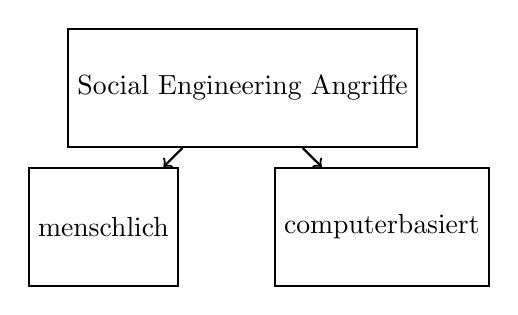
\begin{tikzpicture}[node distance={2.5cm}, thick, main/.style = {draw, rectangle, minimum size=15mm}]
        \node[main] (1) {Social Engineering Angriffe};
        \node[main] (2) [below left of=1] {menschlich};
        \node[main] (3) [below right of=1] {computerbasiert};
        \draw[->] (1) -- (2);
        \draw[->] (1) -- (3);
    \end{tikzpicture}
\end{minipage}
\bcite{1_enisa,4_mdpi}

Andererseits können Angriffsvektoren danach klassifiziert werden, wie die Angriffstechnik ausgeführt wird.
Somit entstehen die folgenden drei Klassifikationen:

\begin{minipage}{.5\linewidth}
    \begin{itemize}
        \setlength\itemsep{1em}
        \item 1) sozial
        \item 2) technisch
        \item 2) physisch
    \end{itemize}
\end{minipage}
\hfill
\begin{minipage}{.5\linewidth}
    \centering
    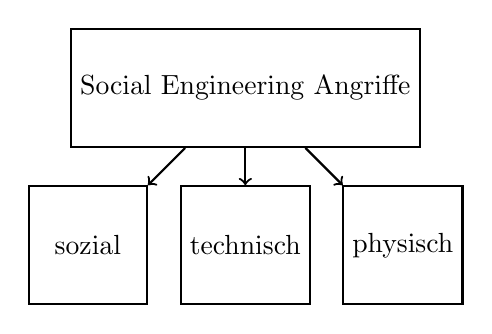
\begin{tikzpicture}[node distance={2cm}, thick, main/.style = {draw, rectangle, minimum size=15mm}]
        \node[main] (1) {Social Engineering Angriffe};
        \node[main] (3) [below of=1] {technisch};
        \node[main] (2) [left of=3] {sozial};
        \node[main] (4) [right of=3] {physisch};
        \draw[->] (1) -- (2);
        \draw[->] (1) -- (3);
        \draw[->] (1) -- (4);
    \end{tikzpicture}
\end{minipage}
\bcite{4_mdpi}

\subsubsection{menschliche Angriffe}
Im Falle von menschlichen Angriffen kommt es durch persönlichen Kontakt zu direkter Interaktion zwischen dem Angreifer und seinem Opfer.
Diese Angriffe können durchaus auch digital ablaufen, etwa über beliebige Messaging-Plattformen, und verwenden gezielte psychologische Manipulation,
die der Angreifer spezifisch auf sein Opfer abstimmt \bcite{4_mdpi, 1_enisa}.

\subsubsection{computerbasierte Angriffe}
Computerbasierte Angriffe, oder auch softwarebasierte Angriffe, werden mithilfe von Computern\footnote{darunter zählen auch Smartphones oder anderweitige computerähnliche Geräte}
ausgeführt, um Informationen des Opfers zu sammeln. Diese Art von Angriff ist in der Lage, eine Vielzahl
von potenziellen Opfern in kürzester Zeit zu erreichen \bcite{4_mdpi, 1_enisa}.

\subsubsection{technische Angriffe}
Technische Angriffe zielen darauf ab, Information wie Passwörter oder Kreditkarteninformationen zu erlangen. Sie werden ausgeführt über das Internet durch die sozialen Medien,
Webseiten oder anderweitigen online Diensten \bcite{4_mdpi,seofwnep}. \qq{Die Kommunikation über digitale Kanäle wie E-Mail bietet ein besonders günstiges Umfeld für Social Engineering.
Während der Täter sein Gegenüber in einer realen Gesprächssituation über alle Sinne hinweg täuschen muss, hat er
es bei der technisch vermittelten Kommunikation deutlich einfacher}\bcite{2_bsi}.

\subsubsection{soziale Angriffe}
Bei sozialen Angriffen werden das psychologische Verhalten und die Emotionen des Opfers ausgenutzt. Diese Angriffe sind am gefährlichsten und in Relation zu ihrer Quantität am
erfolgreichsten, da sie menschlichte Interaktion beinhalten \bcite{4_mdpi}.

\subsubsection{physische Angriffe}
Physische Angriffe definieren diejenigen Aktionen, bei denen der Angreifer selbst materiellen Daten sammelt und nach Informationen sucht.
Beispielsweise durchsucht der Angreifer Mülleimer,
rekonstruiert zerstörte Dokumente oder begeht Diebstahl \bcite{4_mdpi}.

\subsection{Techniken}

Es ist nahezu unmöglich, einen vollständigen Überblick über alle existenten Angriffsvektoren im Bereich des Social Engineering
zu liefern. Wie zuvor in \autoref{chapter:einleitung} erwähnt, sind diverse Social Engineering Techniken mit aktuellen ICT konstant im Wandel.
Etwaige Angriffsmethoden sind wie folgt:

\subsubsection{Phishing}
\label{phishing}
Phishing ist eine der üblichsten Angriffsmethoden des Social Engineering. Es handelt sich um semantische Angriffe durch elektronische
Kommunikationswege (wie etwa E-Mails, HTTP, SMS, VoIP), um manipulative Nachrichten zu übermitteln, die das Opfer dahingehend beeinflussen
sollen, konkrete Aktionen auszuführen. Diese Aktionen beinhalten etwa das Klicken von illegitimen Links oder das Eingeben von (Anmelde-) Informationen.
Die Daten, auf die es ein Angreifer abgesehen hat, erstrecken sich von Kreditkarteninformationen und explizit sensiblen Daten bishin zu Informationen
wie dem Namen eines Elternteils oder Haustieres. Solche Informationen sind oft unscheinbar, können allerdings ein immenses Sicherheitsrisiko
darstellen, etwa im Kontext von Sicherheitsfragen beim Log-in in einen Account. Die am weitesten verbreitete Methode des Phishings ist das
simple Verschicken vorgefertigter E-Mails an zahlreiche Individuen \bcite{4_mdpi,ieee_phishing}.

Phishing Angriffe lassen sich in weitere Unterkategorien einteilen. Darunter liegen zum Beispiel Spear Phishing und Whaling.
Spear Phishing bezieht sich auf Phishing Angriffe, die auf spezifische Individuen oder ausgewählte Gruppen abzielen.
Diese Angriffe sammeln im Vorfeld Informationen, um den Angriff präziser auf ihre Opfer maßzuschneidern. Insofern diese ausgewählten Angriffsziele
hochrangige Persönlichkeiten verkörpern, die als \qqq{Big Fishes} oder \qqq{Whales} bezeichnet werden, handelt es sich um Whaling Angriffe \bcite{4_mdpi}.

Phishing wird im großflächigeren Raum auch als *ishing dargestellt, da die Namensgebung bei dieser Form des Social Engineering abhängig von der
technischen Angriffsmethode ist. So sind beispielsweise Vishing (Voice-Phishing, das Phishing über Telefon), Smishing (SMS-Phishing),
Quishing (QR-Code-Phishing) oder Tishing (Microsoft-Teams-Phishing) definiert \bcite{verizon2024}.

\subsubsection{Pretexting}
\label{pretexting}
Diese Technik verwendet einen Vorwand (engl. \qqq{Pretext}), also eine falsche Rechtfertigung für eine bestimmte Vorgehensweise, um das Vertrauen des
Opfers zu gewinnen und dieses zur Kooperation zu manipulieren. Pretexting zielt auf die Emotionen des Opfers ab, um neben Vertrauen ein Gefühl von
Dringlichkeit oder Sympathie zu erzeugen. Das Hauptmerkmal dieses Angriffes ist seine kreative Komponente. Oftmals täuschen Cyber-Kriminelle
eine Autoritätsperson vor, wie etwa einen Investor, und legen sogar fälschliche online Persona mitsamt Webseiten und Bewertungen an, um seriös zu wirken.
Populär ist auch das Ausgeben als IT support mit der Anfrage auf Log-in Daten, welche angeblich zu Wartungszwecken gebraucht werden.
Andere Methoden enthalten Romance-Scams, in denen der Betrüger ein Interesse an einer romantischen Beziehung vorspielt, oder Nachahmung, wobei der
Angreifer sich zum Beispiel als Firmenkollege ausgibt und das Opfer um \qq{dringende Hilfe} bittet \bcite{1_enisa,4_mdpi}.

\subsubsection{Tailgaiting}
\label{tailgating}
Unter Tailgating versteht man das physische Eindringen eines Social Engineers in unbefugte Areale.
Dies wird erreicht, indem der Kriminelle Personen mit Sicherheitsbefugnis dicht folgt, Sperrzonen bewusst umgeht oder Pretexting (\autoref{pretexting})
verwendet. Beispielsweise erklären Angreifer selbstbewusst, dass sie ID Karte verloren oder vergessen haben. In vielen Szenarien wird die
Befugnis durch das äußere Erscheinungsbild, wie zum Beispiel dem Tragen von Warnwesten oder dem Dresscode eines Unternehmens vorgetäuscht oder die Hilfsbereitschaft anderer ausgenutzt,
indem der Angreifer zum Beispiel schwere/viele Boxen trägt. Insofern im Prozess des Angriffes die Erlaubnis von befugtem Personal erlangt wird, handelt es sich um sogenanntes Piggybacking \bcite{4_mdpi}.

\subsubsection{Baiting}
\label{baiting}
Baiting ist eine Social Engineering Methode, die sich die Neugierde der Menschen zunutze macht.
Sie zeichnet sich dadurch aus, bewusst einfachen Zugang zu einem Köder zu bieten, welcher darauf abzielt, eine konkrete Handlung
des Opfers auszulösen. Im Kontext der Phishing Angriffe lädt eine Baiting E-Mail etwa dazu ein, auf einen Link zu klicken, der beispielsweise
kostenlose Prämien verspricht. Unter Baiting Angriffe fallen ebenfalls sogenannte Media-Drops. Beispielsweise werden bei USB-Drops absichtlich
USB-Sticks platziert, die darauf abzielen, gefunden zu werden, und bei Verwendung den Computer infizieren. Eine weitere Möglichkeit ist es, die
infizierten Medien wie CDs oder anderweitige beliebige Datenträger vor Firmengeländen als Werbegeschenke zu verteilen. Bei erfolgreicher Infektion eines Computers haben die Akteure bereits
die Möglichkeit, Informationen zu stehlen oder anderweitige Malware zu installieren; beliebt sind Trojaner zu langzeitlichen Kontrolle eines
Systems, Ransomware als Form der Erpressung \bcite{1_enisa,4_mdpi,ransomware} oder Spyware zur kontinuierlichen Informationssammlung.

\subsubsection{Quid Pro Quo}
Quid pro quo (lateinisch für \qqq{dies für das}) funktioniert auf eine ähnliche Weise wie Baiting Angriffe, wobei dieser Angriffsvektor nicht
Neugierde, sondern Vertrauen ausnutzt. Es handelt sich um eine Anfrage nach persönlichen oder geschäftlichen Informationen im Austausch gegen Kompensation.
Angreifer bieten zumeist einen Service an, der für das Opfer verlockend oder hilfreich ist. Quid Pro Quo wird oftmals in gezielten
Spear Phishing Angriffen (\autoref{phishing}) verwendet. Möglich ist auch, dass der Angreifer eine Studie oder ein Experiment vortäuscht, was bei Teilnahme Kontaktdaten
benötigt und im Gegenzug eine Geldsumme verspricht \bcite{1_enisa}.

\subsubsection{Reverse Social Engineering}
Reverse Social Engineering Angriffe lassen ihre Opfer glauben, es gäbe ein (technisches) Problem oder inszenieren einen tatsächlichen Schaden, wenn sie beispielsweise
ein Netzwerk zum Absturz bringen. Im Folgenden überzeugen sie ihre Opfer auf verschiedenste Weise, dass sie alleine das Problem beheben können. Während sie das Problem
lösen, erlangen sie die gewünschten Informationen und ziehen sich abschließend zurück, ohne jemals ihre Identität preiszugeben \bcite{4_mdpi}.
Im Gegensatz zu anderen Social Engineering Angriffen sind es nicht die Angreifer, die auf ihre Opfer zugehen, sondern die Opfer, die gutgläubig Hilfe
bei den Angreifern suchern.

\subsubsection{Pop-Up Windows}
Es existieren zwei verschiedene Grundstrukturen im Aufbau von Pop-up Fenstern als Social Engineering Taktik. Erstere verwendet eine Methodik ähnlich zum Baiting (\autoref{baiting}).
Hierbei wird zum Beispiel vorgetäuscht, das potenzielle Opfer habe in einer Verlosung oder der Lotterie gewonnen.
Zweitere verwendet elementar die Taktik von Scareware; es wird also Panik beim Opfer ausgelöst, mit dem Ziel, dieses verängstigt in unüberlegte Handlungen zu bewegen. Die hierbei
dargestellte Gefahr wirkt bedrohlich, ist allerdings lediglich simuliert und nicht existent. Unter den populärsten Pop-up-Windows sind fälschliche Nachrichten, die davon
überzeugen sollen, der Computer habe bereits Malware installiert und benötige nun ein Antivirenprogramm, welches im selbigen Pop-Up Fenster angeboten wird.
Insgesamt lassen sich derartige Angriffe primär eingebunden in Webseiten finden, durch (Browser-) Plug-ins oder
zuvor installierten Programmen. Das Ziel dieser Fenster ist es, dazu zu bewegen, Informationen einzugeben, auf Links zu klicken oder Fake Software\footnote{Fake Software enthält oft zu teilen legitime Software, welche der Social Engineer neu verpackt} herunterzuladen.

\subsubsection{Weiteres}
Es gibt viele weitere Arten von Angriffsvektoren. Einige davon lassen sich wie folgt zusammenfassen:

\begin{itemize}
    \setlength\itemsep{-1em}
    \item Impersonation/Masquerading: Eine Form des Identitätsdiebstahles, bei der der Angreifer vorgibt jemand anderes zu sein.
    \item Eavesdropping: Das unbemerkte Mithören, oder Lesen, von der Kommunikation Anderer, ohne deren Erlaubnis.
    \item Shoulder surfing: Das Beobachten von Personen, während diese sensible Daten, wie Passwörter, eingeben.
    \item Dumpster diving: Der Angreifer sammelt sensible Informationen, wie (geschredderte) Dokumente, in dem Mülleimern seines Ziels.
    \item Diversion Theft: Ein Transportunternehmen, oder -vehikel, wird mit falschen Anweisungen beauftragt, ein Paket an einen vom Kriminellen gewünschten Ort zu bringen.
    \item Pharming: Der Datenverkehr einer Webseite wird auf eine andere, bösartige Webseite umgeleitet.
    \item Deepfake: Medien, die künstlich verändert oder generiert werden, um den fälschlichen Anschein zu erwecken, dass Individuen etwas getan oder gesagt haben.
\end{itemize}

\bcite{4_mdpi,ceh}
